% ***********************************************************
% ******************* PHYSICS HEADER ************************
% ***********************************************************
% Version 2
\documentclass[11pt]{article}
\usepackage{amsmath} % AMS Math Package
\usepackage{amsthm} % Theorem Formatting
\usepackage{amssymb}	% Math symbols such as \mathbb
\usepackage{graphicx} % Allows for eps images
\usepackage{multicol} % Allows for multiple columns
\usepackage[dvips,letterpaper,margin=0.75in,bottom=0.5in]{geometry}
\usepackage{authblk} % Allows for authors from multiiple institutes
\renewcommand\Authands{ and } % for authblk
\usepackage{indentfirst} % to have indent for the 1st paragraph of each section

 % Sets margins and page size
\pagestyle{empty} % Removes page numbers

\makeatletter % Need for anything that contains an @ command

\newcommand{\affil}[1]{\def\@affilname{#1}}
\def\@affil{\@affilname}

\renewcommand{\maketitle} % Redefine maketitle to conserve space
{ \begingroup \vskip 10pt \begin{center} \large {\textbf{\@title}}
\vskip 10pt \large \@author \vskip 10pt \large \@affil \end{center}
\vskip 10pt \endgroup \setcounter{footnote}{0} }

\makeatother % End of region containing @ commands
\renewcommand{\labelenumi}{(\alph{enumi})} % Use letters for enumerate
% \DeclareMathOperator{\Sample}{Sample}
\let\vaccent=\v % rename builtin command \v{} to \vaccent{}
\renewcommand{\v}[1]{\ensuremath{\mathbf{#1}}} % for vectors
\newcommand{\gv}[1]{\ensuremath{\mbox{\boldmath$ #1 $}}}
% for vectors of Greek letters
\newcommand{\uv}[1]{\ensuremath{\mathbf{\hat{#1}}}} % for unit vector
\newcommand{\abs}[1]{\left| #1 \right|} % for absolute value
\newcommand{\avg}[1]{\left< #1 \right>} % for average
\let\underdot=\d % rename builtin command \d{} to \underdot{}
\renewcommand{\d}[2]{\frac{d #1}{d #2}} % for derivatives
\newcommand{\dd}[2]{\frac{d^2 #1}{d #2^2}} % for double derivatives
\newcommand{\pd}[2]{\frac{\partial #1}{\partial #2}}
% for partial derivatives
\newcommand{\pdd}[2]{\frac{\partial^2 #1}{\partial #2^2}}
% for double partial derivatives
\newcommand{\pdc}[3]{\left( \frac{\partial #1}{\partial #2}
 \right)_{#3}} % for thermodynamic partial derivatives
\newcommand{\ket}[1]{\left| #1 \right>} % for Dirac bras
\newcommand{\bra}[1]{\left< #1 \right|} % for Dirac kets
\newcommand{\braket}[2]{\left< #1 \vphantom{#2} \right|
 \left. #2 \vphantom{#1} \right>} % for Dirac brackets
\newcommand{\matrixel}[3]{\left< #1 \vphantom{#2#3} \right|
 #2 \left| #3 \vphantom{#1#2} \right>} % for Dirac matrix elements
\newcommand{\grad}[1]{\gv{\nabla} #1} % for gradient
\let\divsymb=\div % rename builtin command \div to \divsymb
\renewcommand{\div}[1]{\gv{\nabla} \cdot #1} % for divergence
\newcommand{\curl}[1]{\gv{\nabla} \times #1} % for curl
\let\baraccent=\= % rename builtin command \= to \baraccent
\renewcommand{\=}[1]{\stackrel{#1}{=}} % for putting numbers above =
\newtheorem{prop}{Proposition}
\newtheorem{thm}{Theorem}[section]
\newtheorem{lem}[thm]{Lemma}
\theoremstyle{definition}
\newtheorem{dfn}{Definition}
\theoremstyle{remark}
\newtheorem*{rmk}{Remark}

\usepackage[english]{babel}
\graphicspath{{images/}}
\usepackage{siunitx}
\usepackage{lineno}

\def\lycoris{\textsc{Lycoris }}%
\def\GeV{\ifmode {\mathrm{\ Ge\kern -0.1em V }}\else
								 {\textrm{Ge\kern -0.1em V }}\fi}%

% ***********************************************************
% ********************** END HEADER *************************
% ***********************************************************


\begin{document}

\title{\textsc{Lycoris}: A large area beam telescope based on hybrid-less strip silicon sensors}
\author[*]{Mengqing Wu}
\author[*]{Uwe Kraemer}
\author[*]{Marcel Stanitziki}
\author[**]{Martin Breidenbach}
\author[**]{Dietrich R. Freytag}
\author[**]{Benjamin A. Reese}
\affil[*]{Deutsches Elektronen-Synchrotron DESY, Notkestr. 85, 22607 Hamburg, Germany}
\affil[**]{Stanford Linear Accelerator Center SLAC, 2575 Sand hill Rd, Menlo Park, CA 94025 USA}

\maketitle

\begin{abstract}
%\linenumbers

A new Large area x-Y COverage Readout Integrated Strip telescope (\lycoris) is being built to address user demands,
as an improvement of the DESY test beam infrastructure within the Advanced European Infrastructures for Detectors at Accelerators project (AIDA-2020).
The \lycoris consists of 6 layers of \SI{25}{\micro\metre} pitch strip Si sensor readout by 2 bump-bonded ASICs (KPiX),
running at a timing resolution as multiples of \SI{80}{\nano\second};
its active area is designed to be 10$\times$\SI{10}{\square\centi\metre}, extendable to 10$\times$\SI{20}{\square\centi\metre}.
It will be mounted inside a \SI{1}{\tesla} solenoid magnet,
providing a spatial resolution better than \SI{10}{\micro\metre} along the bending direction,
and a resolution better than \SI{1}{\milli\meter} along the magnetic field.
The full readout system was tested with a hexagonal pixel sensor in the lab with a Sr90 source,
and later tested in the electron beam at DESY in May and October 2017;
the first assembled modules were tested in the spring 2018.
First results of the \lycoris prototype will be presented with a comparison to simulation,
besides, the characterization of sensor and readout system are also included.
\end{abstract}

\section*{A large active area beam telescope}
%\linenumbers

DESY test beam facility provides $e^-/e^+$ beams with energies from 1 to \SI{6}{\GeV} up to \SI{1}{\MHz}
%converted from bremsstrahlung beams from carbon fibre targets in the electron-positron synchrotron DESY II,
with three test beam lines (21, 22 and 24).
The beam lines 21 and 22 are both equiped with a EUDET-type beam telescope~$^{\cite{eudet}}$ with an active area of around 1$\times$\SI{2}{\square\centi\metre},
which is based on a fine pitch \uppercase{mimosa}~26 monolithic sensor with an event readout frame of \SI{115.2}{\micro\second};
the beam line 24 is equiped with a \SI{1}{\tesla} solenoid, namely PCMAG, at a diameter of $\sim$\SI{85}{\centi\metre} with its wall of $\sim20X_0$,
inside which both the EUDET-type telescope and the Device Under Test (DUT) can be inserted.
The EUDET-type beam telescope at DESY is proven to meet user's demands very well and thus in a high ($\sim$70\%) demand,
however, its active area is limited to cover the bending curvature for PCMAG users.
Therefore, the \lycoris telescope is designed to have a large active area of 10$\times$\SI{10}{\square\centi\metre}, extendable to 10$\times$\SI{20}{\square\centi\metre},
in order to cover 90\% to 96\% particles with energies from 1 to \SI{6}{\GeV}.

\begin{figure}[!ht]%
\centering
%\vspace{-10px}
\hspace{-100px}
\parbox{1.2in}{
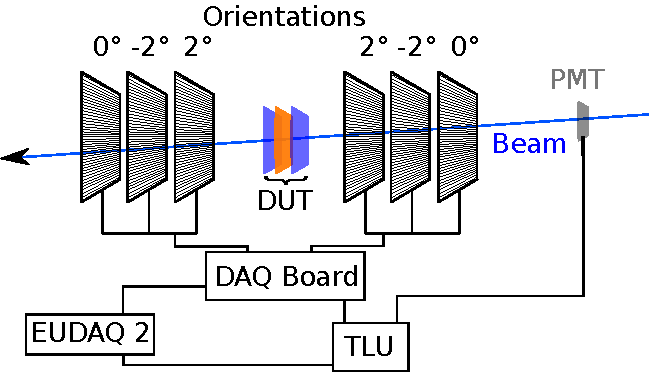
\includegraphics[width=2.5\linewidth]{pics/principle.pdf}
}%
\hspace{150px}
\begin{minipage}{1.2in}%
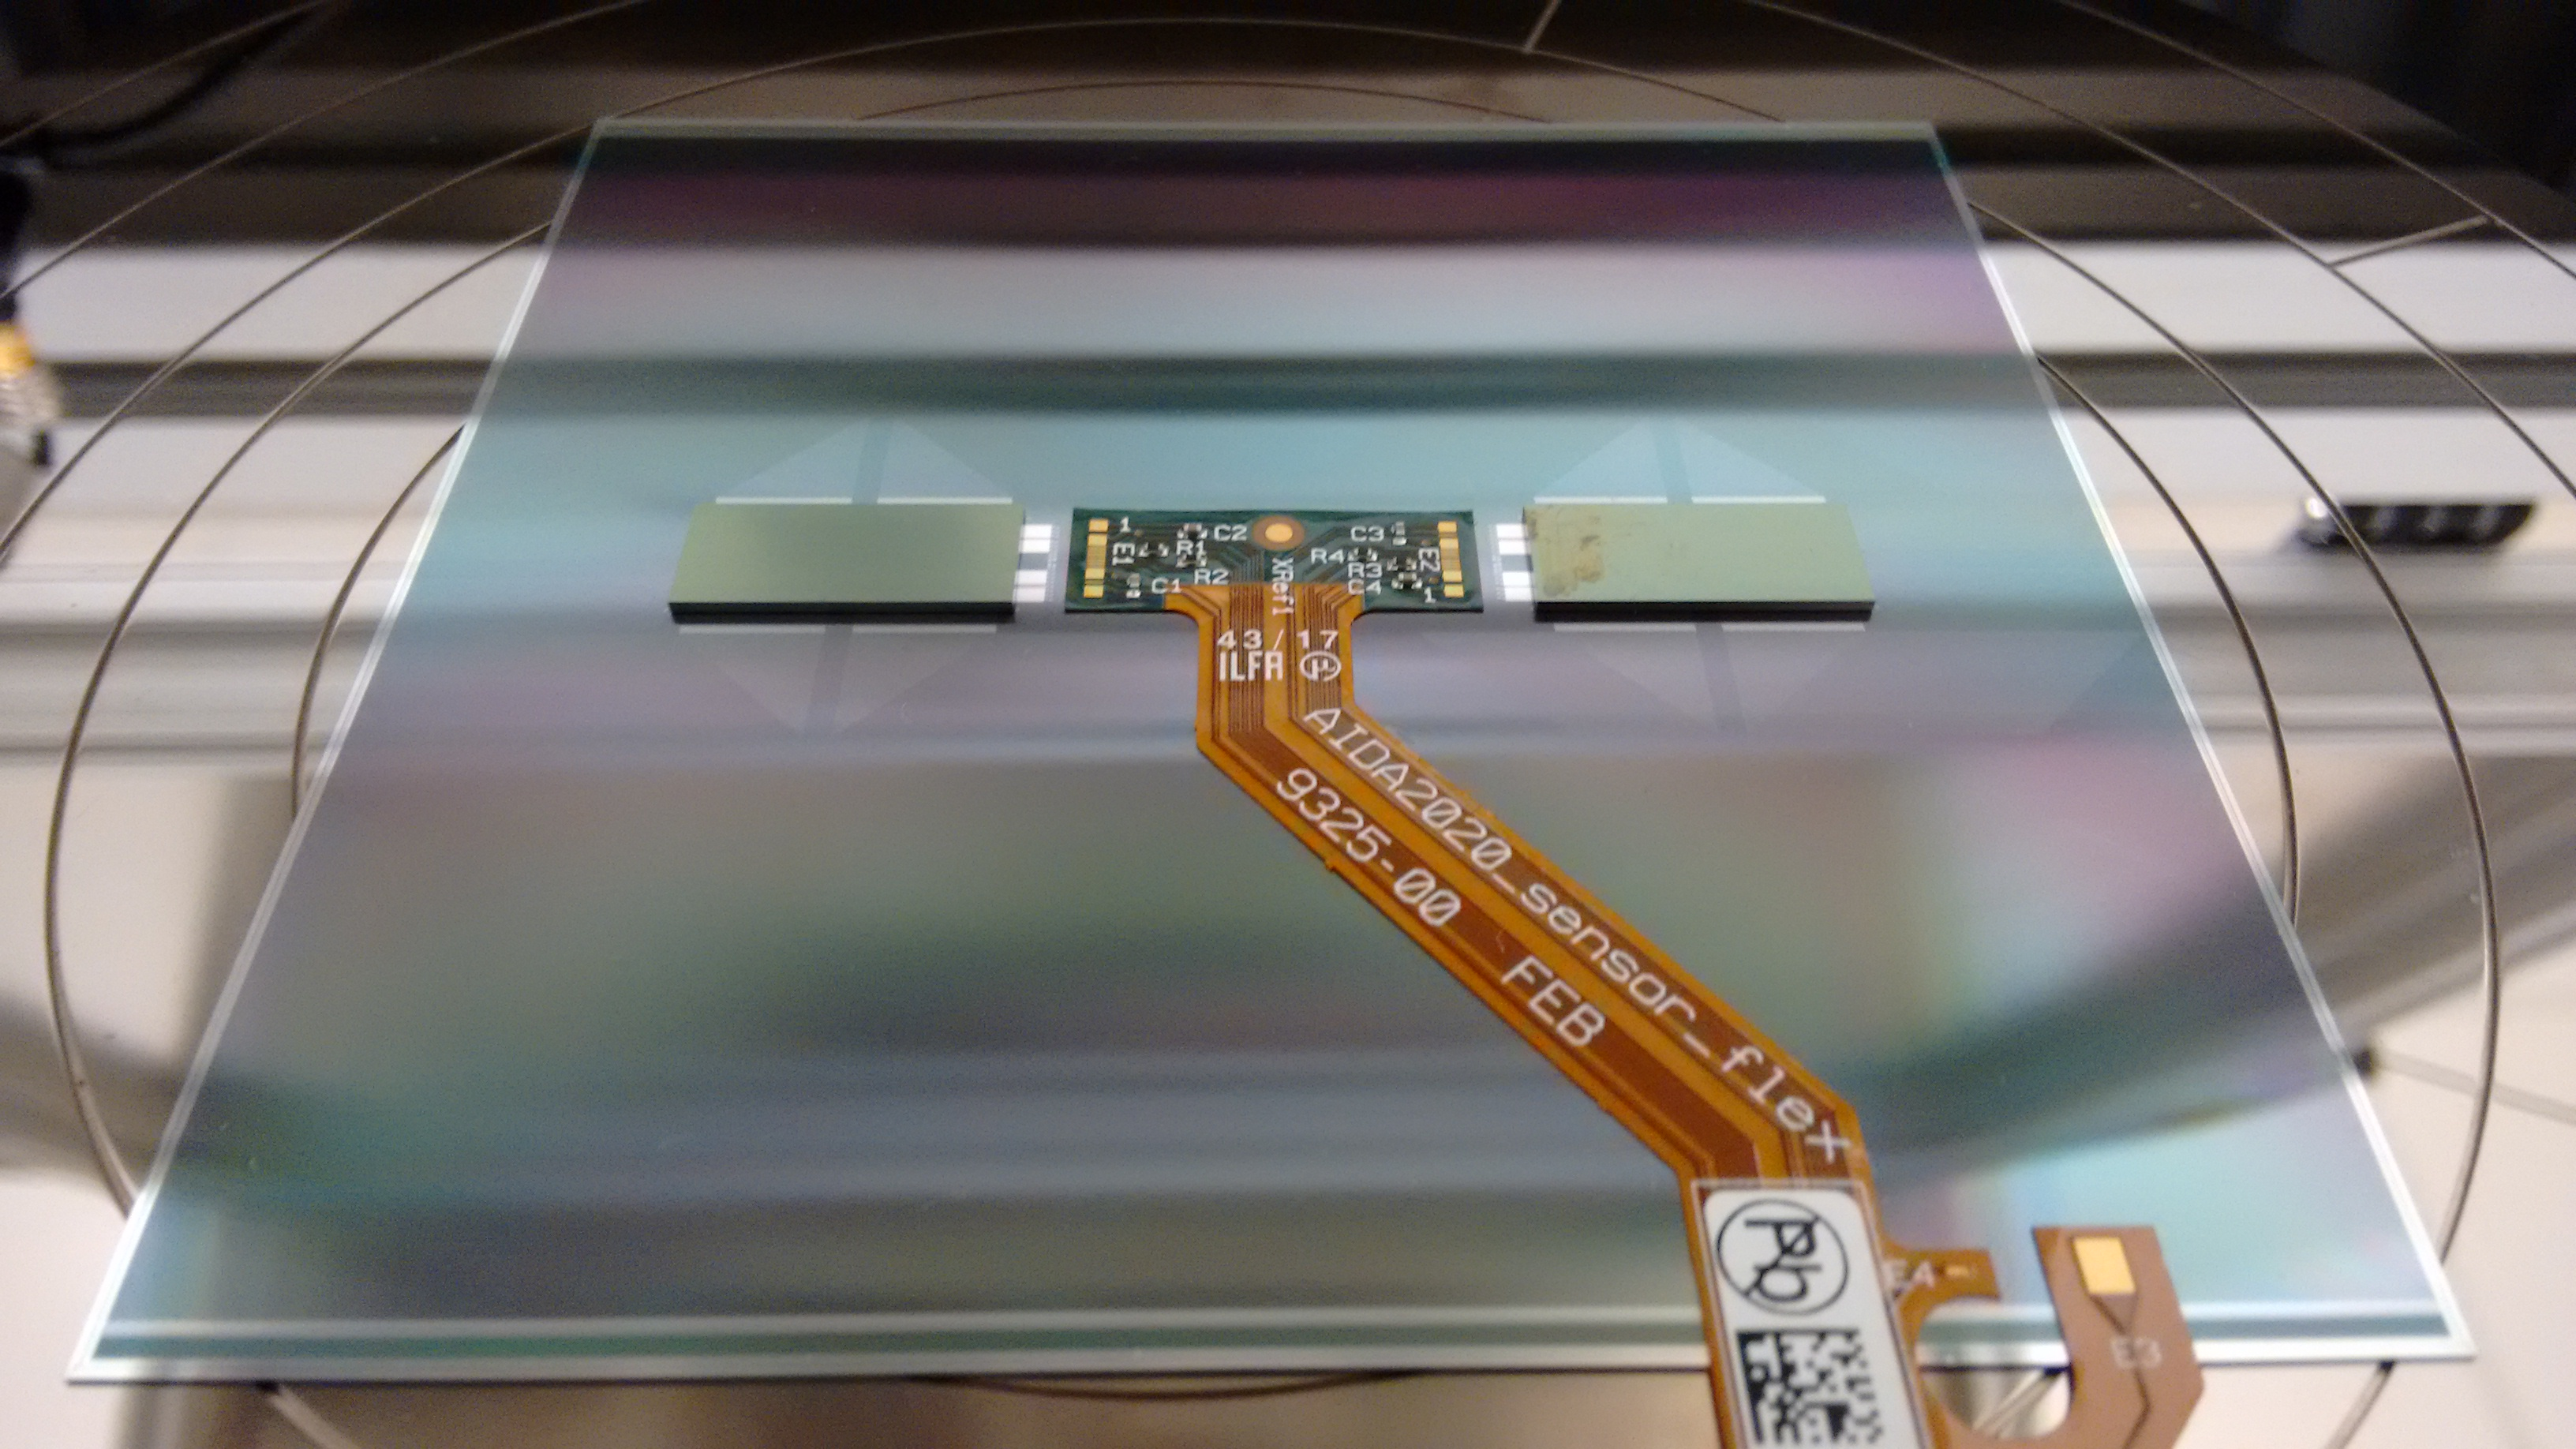
\includegraphics[width=2.5\linewidth]{pics/sensor_module1.jpg}
\end{minipage}%
\caption{On the left, testbeam setup used at the CERN SPS in Summer 2015. On the right, picture of the AHCAL testbeam prototype used at the CERN SPS in Summer 2015. The front face of the calorimeter is on the right of the picture.}%
\label{fig:1figs}%
\end{figure}


\begin{figure}[!ht]%
\centering
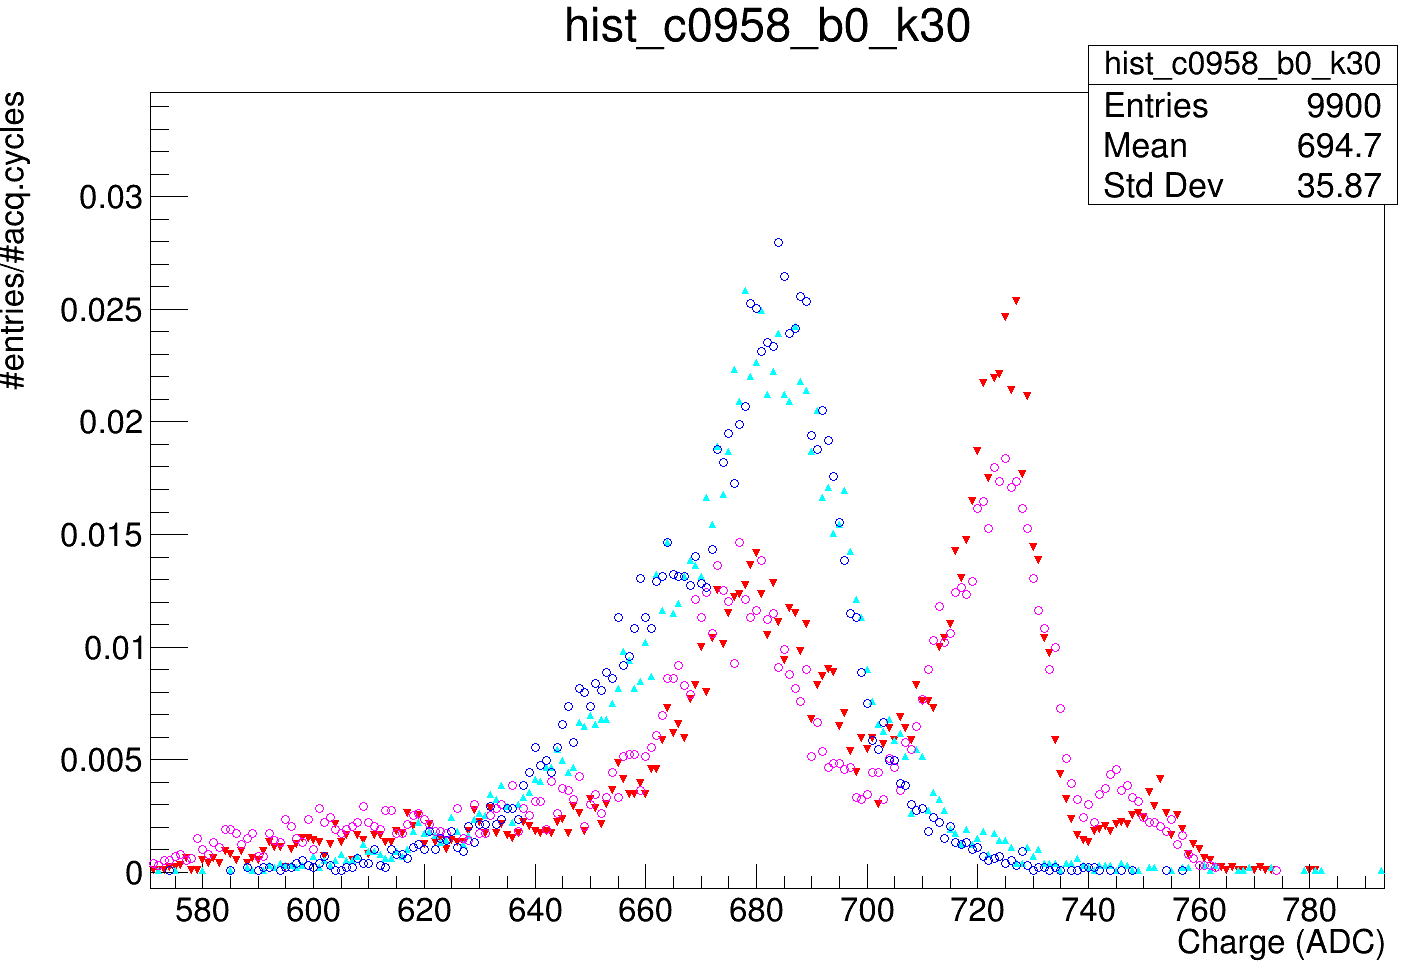
\includegraphics[width=0.49\linewidth]{pics/hist1.jpg}
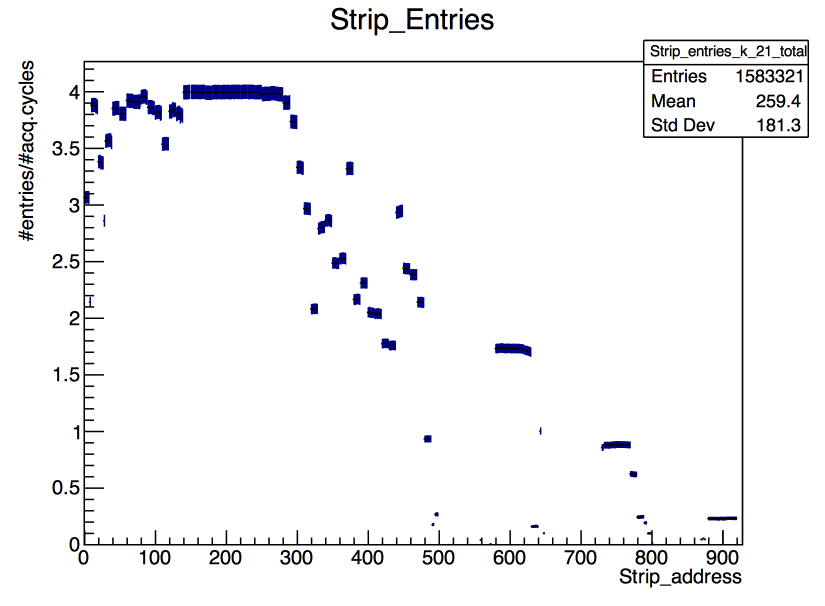
\includegraphics[width=0.49\linewidth]{pics/S58_K2_2018_05_07_16_49_42_strip_entries.png}
\caption{}%
\label{fig:2figs}%
\end{figure}

Blah more details here.

Plan and target to show.

In this contribution, we will describe the latest \lycoris prototype, and we will present the first results on testing the prototype with comparison to simulation, as well as the sensor and readout system characterization.

\footnotesize
\begin{thebibliography}{1}

\bibitem{eudet} H.~Jansen et al., {\em Performance of the EUDET-type beam telescopes},
\textbf{EPJ Tech.\ Instrum.\  {\bf 3}, no. 1, 7 (2016)}.

\bibitem{lycoris1} U.~Kraemer et al., {\em LYCORIS - A Large Area Strip Telescope},
\textbf{arXiv:1801.08505 [physics.ins-det]}.

%\bibitem{mimosa} J.~Baudot et al., {\em First test results Of MIMOSA-26, a fast CMOS sensor with integrated zero suppression and digitized output},
%\textbf{2009 IEEE Nuclear Science Symposium Conference Record (NSS/MIC), Orlando, FL, 2009, pp. 1169-1173}.

\bibitem{T3B} The CALICE Collaboration, C. Adloff et al., {\em The time structure of hadronic showers in highly granular calorimeters with tungsten and
steel absorbers}, \textbf{2014 JINST 9 P07022}.

\end{thebibliography}

\end{document}
